\documentclass[pre,aps,superscriptaddress,nofootinbib]{revtex4}

\usepackage{amsmath,amsfonts,amssymb,bm,graphicx,hyperref,listings,xcolor,float}
\setlength{\parindent}{0pt}

\begin{document}

\title{2 RTPs on a ring}
\author{Yann-Edwin Keta}
\maketitle

% \maketitle

\nocite{Slowman2016, Nemoto2016, Chetrite2015}

\section{Model}

\subsection{Fokker-Planck equations}

We consider 2 run-and-tumble particles (RTPs), with swim speed $v_0$ and tumble rate $\tau^{-1}$ on a linear ring of length $L$. With $r_1, r_2 \in [0, L]$ the positions and $\alpha_1, \alpha_2 = \pm$ the states of each particles, and $V(r_1, r_2) = V(|r_1 - r_2|)$ the potential of interactions between these particles, we have the equations of motion
\begin{equation}
\dot{r}_i = \alpha_i v_0 - \partial_{r_i} V(|r_1 - r_2|)
\label{EOM}
\end{equation}
and the Fokker-Planck equations for the joint distribution of positions
\begin{equation}
\begin{aligned}
\dot{P}_{\alpha_1, \alpha_2}(r_1, r_2) =
  &- v_0(\alpha_1 \partial_{r_1} + \alpha_2 \partial_{r_2}) P_{\alpha_1\alpha_2}(r_1, r_2)
    &&\to \text{Propulsion}\\
  &+ \partial_{r_1} (P_{\alpha_1\alpha_2}(r_1, r_2)\partial_{r_1}V(|r_1 - r_2|))
    &&\to \text{Interaction}\\
  &+ \partial_{r_2} (P_{\alpha_1\alpha_2}(r_1, r_2)\partial_{r_2}V(|r_1 - r_2|))
    &&\\
  &+ \tau^{-1} (P_{\overline{\alpha_1}\alpha_2}(r_1, r_2) + P_{\alpha_1\overline{\alpha_2}}(r_1, r_2) - 2 P_{\alpha_1\alpha_2}(r_1, r_2))
    &&\to \text{Tumble}\\
  =& \, \mathcal{L}^{\dagger}_{\alpha_1\alpha_2} P_{\alpha_1\alpha_2}(r_1, r_2)
\end{aligned}
\label{FP0}
\end{equation}
with $\mathcal{L}^{\dagger}_{\alpha_1\alpha_2}$ the Fokker-Planck operator.\\

We introduce $r \equiv r_2 - r_1 \geq 0$, such that $\partial_{r_1} \equiv - \partial_r$ and $\partial_{r_2} = \partial_r$, with which we can define the symmetries
\begin{eqnarray}
\label{evensymmetry}
P_{++}(r) = P_{--}(r),\\
\label{oddsymmetry}
P_{+-}(r) = P_{-+}(L - r),
\end{eqnarray}
and the interaction potential
\begin{align*}
V(r) = \begin{cases} 0 &\text{ if } r \in ]0, L[ \\ \infty &\text{ otherwise} \end{cases}
\end{align*}
such that, with Eq. (\ref{EOM}), we get for particles with opposite directions
\begin{equation}
- \partial_r V(0) = \partial_r V(L) = v_0.
\end{equation}
because of mutual hindrance.\\

We can solve the steady state problem with the normalisation condition
\begin{equation}
\int_0^L \mathrm{d}r \, \sum_{\alpha_1\alpha_2} P_{\alpha_1\alpha_2}(r) = 1
\label{normalisation}
\end{equation}
the bulk equations
\begin{equation}
\dot{P}_{\alpha_1\alpha_2}(r \in ]0, L[) = 0
\label{bulk}
\end{equation}
the left boundary equations
\begin{equation}
\int_{0^-}^{0^+} \mathrm{d}r \, \dot{P}_{\alpha_1\alpha_2}(r) = 0
\label{leftboundary}
\end{equation}
and the right boundary equations
\begin{equation}
\int_{L^-}^{L^+} \mathrm{d}r \, \dot{P}_{\alpha_1\alpha_2}(r) = 0.
\label{rightboundary}
\end{equation}

\subsection{Biased ensemble}

We define our biasing quantity
\begin{equation}
\dot{Z} = \sum_{i=1}^2 - \partial_{r_i} V(r) \alpha_i v_0 = v_0 (\alpha_1 - \alpha_2) \partial_r V(r)
\end{equation}
which is non-zero only at contact, and the tilted generator
\begin{equation}
\mathcal{W}^{\dagger}_{\alpha_1\alpha_2} = \mathcal{L}^{\dagger}_{\alpha_1\alpha_2} - s \dot{Z}
\end{equation}
with $s$ the biasing parameter, which eigenvalue problem
\begin{equation}
\psi P_{\alpha_1\alpha_2}(r) = \mathcal{W}^{\dagger}_{\alpha_1\alpha_2} P_{\alpha_1\alpha_2}(r)
\label{eigenproblem}
\end{equation}
we have to solve for $\psi(s)$ its largest eigenvalue, which defines the dynamical free energy.\\

While the symmetries (Eqs. (\ref{evensymmetry}, \ref{oddsymmetry})) and the normalisation condition (Eq. (\ref{normalisation})) remains unchanged, we have that the bulk equations (Eq. (\ref{bulk})), the left boundary equations (Eq. \ref{leftboundary}), and the right boundary equations (Eq. \ref{rightboundary}) become
\begin{eqnarray}
\label{bulk:biased}
\psi P_{\alpha_1\alpha_2}(r \in ]0, L[) = \mathcal{W}^{\dagger}_{\alpha_1\alpha_2} P_{\alpha_1\alpha_2}(r \in ]0, L[)\\
\label{leftboundary:biased}
\int_{0^-}^{0^+} \mathrm{d}r \, \psi P_{\alpha_1\alpha_2}(r) = \int_{0^-}^{0^+} \mathrm{d}r \, \mathcal{W}^{\dagger}_{\alpha_1\alpha_2} P_{\alpha_1\alpha_2}(r)\\
\label{rightboundary:biased}
\int_{L^-}^{L^+} \mathrm{d}r \, \psi P_{\alpha_1\alpha_2}(r) = \int_{L^-}^{L^+} \mathrm{d}r \, \mathcal{W}^{\dagger}_{\alpha_1\alpha_2} P_{\alpha_1\alpha_2}(r)
\end{eqnarray}
respectively.

\section{Unbiased steady state distribution}

We use the following ansatz for the unbiased ($s = 0$) steady state distribution
\begin{equation}
P_{\alpha_1\alpha_2}(r) = a_{\alpha_1\alpha_2} + b_{\alpha_1\alpha_2} \delta(r) + c_{\alpha_1\alpha_2} \delta(L - r)
\end{equation}
which satisfies the normalisation condition (Eq. (\ref{normalisation}))
\begin{equation}
\sum_{\alpha_1\alpha_2} \left(L a_{\alpha_1\alpha_2} + b_{\alpha_1\alpha_2} + c_{\alpha_1\alpha_2}\right) = 1
\end{equation}
the bulk equations (Eq. (\ref{bulk}))
\begin{eqnarray}
\tau^{-1} (a_{+-} + a_{-+} - 2 a_{++}) = 0\\
\tau^{-1} (a_{+-} + a_{-+} - 2 a_{--}) = 0\\
\tau^{-1} (a_{++} + a_{--} - 2 a_{+-}) = 0\\
\tau^{-1} (a_{++} + a_{--} - 2 a_{-+}) = 0
\end{eqnarray}
the left boundary equations (Eq. (\ref{leftboundary}))
\begin{eqnarray}
\tau^{-1}(b_{+-} + b_{-+} - 2 b_{++}) = 0\\
\tau^{-1}(b_{+-} + b_{-+} - 2 b_{--}) = 0\\
2 v_0 a + \tau^{-1}(b_{++} + b_{--} - 2 b_{+-}) = 0\\
- 2 v_0 a + \tau^{-1}(b_{++} + b_{--} - 2 b_{-+}) = 0
\end{eqnarray}
the right boundary equations (Eq. (\ref{rightboundary}))
\begin{eqnarray}
\tau^{-1}(c_{+-} + c_{-+} - 2 c_{++}) = 0\\
\tau^{-1}(c_{+-} + c_{-+} - 2 c_{--}) = 0\\
- 2 v_0 a + \tau^{-1}(c_{++} + c_{--} - 2 c_{+-}) = 0\\
2 v_0 a + \tau^{-1}(c_{++} + c_{--} - 2 c_{-+}) = 0
\end{eqnarray}
and the symmetries (Eqs. (\ref{evensymmetry}, \ref{oddsymmetry})).\\

We get
\begin{eqnarray}
\label{s0++}
P_{++}(r) = a + l a \delta(r) + l a \delta(L - r)\\
\label{s0--}
P_{--}(r) = a + l a \delta(r) + l a \delta(L - r)\\
\label{s0+-}
P_{+-}(r) = a + 2 l a \delta(r)\\
\label{s0-+}
P_{-+}(r) = a + 2 l a \delta(L - r)
\end{eqnarray}
with
\begin{equation}
a = \frac{1}{4(L + 2l)}
\label{smooth_unbiased}
\end{equation}
and the persistence length $l = v_0 \tau$.

\section{Biased steady state distribution}
\label{sec:biased-distribution}

\subsection{Exact solution}

We use the following ans\"atze for the steady state distribution
\begin{eqnarray}
P_{++}(r) = P_{--}(r) = \beta(r) + \gamma_- \delta(r) + \gamma_+ \delta(L - r)\\
P_{+-}(r) = \varepsilon(r) + \zeta \delta(r)\\
P_{-+}(r) = \theta(r) + \zeta \delta(L - r)\\
\end{eqnarray}
with $\varepsilon(r) = \theta(L - r)$ according to Eq. (\ref{oddsymmetry}).\\

We write the eigenvalue equations (Eq. (\ref{eigenproblem}))
\begin{eqnarray}
\label{FP1}
\psi P_{\alpha\alpha}(r) = 2 \partial_r(P_{\alpha\alpha}(r) \partial_r V(r)) + \tau^{-1} (P_{+-}(r) + P_{-+}(r) - 2 P_{\alpha\alpha}(r))\\
\label{FP2}
\psi P_{+-}(r) = 2 v_0 \partial_r P_{+-}(r) + 2 \partial_r(P_{+-}(r) \partial_r V(r)) + \tau^{-1}(2 P_{\alpha\alpha}(r) - 2 P_{+-}(r)) - 2 s v_0 \partial_r V(r) P_{+-}(r)\\
\label{FP3}
\psi P_{-+}(r) = - 2 v_0 \partial_r P_{-+}(r) + 2 \partial_r(P_{-+}(r) \partial_r V(r)) + \tau^{-1}(2 P_{\alpha\alpha}(r) - 2 P_{-+}(r)) + 2 s v_0 \partial_r V(r) P_{-+}(r)
\end{eqnarray}
and integrate from Eqs. (\ref{FP1}, \ref{FP2}, \ref{FP3}) the sum of $\psi(2 P_{\alpha\alpha} + P_{+-} + P_{-+})$ between $0^-$ and $L^+$ to get
\begin{equation}
\psi = 4 s v_0 \partial_r V(L) \zeta = 4 s v_0^2 \zeta
\label{psiZeta}
\end{equation}
linking the dynamical free energy $\psi$ and the sticking term $\zeta$.\\

We have the bulk equations (Eq. (\ref{bulk:biased}))
\begin{eqnarray}
\label{bulk:biased1}
\psi \beta(r) = \tau^{-1} (\varepsilon(r) + \theta(r) - 2 \beta(r))\\
\label{bulk:biased2}
\psi \epsilon(r) = 2 v_0 \varepsilon^{\prime}(r) + \tau^{-1} (2 \beta(r) - 2 \varepsilon(r))\\
\label{bulk:biased3}
\psi \theta(r) = -2 v_0 \theta^{\prime}(r) + \tau^{-1} (2 \beta(r) - 2 \theta(r))
\end{eqnarray}
such that Eq. (\ref{bulk:biased1}) gives
\begin{equation}
\beta(r) = (2 + \tau\psi)^{-1} (\epsilon(r) + \theta(r))
\end{equation}
and the difference and sum of Eqs. (\ref{bulk:biased2}, \ref{bulk:biased3}) give
\begin{eqnarray}
2 l (\varepsilon(r) + \theta(r))^{\prime} = (2 + \tau \psi)(\varepsilon(r) - \theta(r))\\
\begin{aligned}
2 l (\varepsilon(r) - \theta(r))^{\prime} &= -4 \beta(r) + (\tau\psi + 2)(\varepsilon(r) + \theta(r))\\
&= \left((\tau\psi + 2) - \frac{4}{\tau\psi + 2}\right)(\varepsilon(r) + \theta(r))
\end{aligned}
\end{eqnarray}
where we set $A(r) = \varepsilon(r) + \theta(r)$ and $B(r) = \varepsilon(r) - \theta(r)$, which on the one hand verify
\begin{equation}
A^{\prime\prime}(r) - k^2 A(r) = 0
\end{equation}
where
\begin{equation}
k^2 l^2 = \tau \psi \left(\frac{\tau \psi}{4} + 1\right)
\label{kPsi}
\end{equation}
and which general solution is
\begin{equation}
A(r) = A_+ e^{- k r} + A_- e^{-k (L - r)}
\end{equation}
and on the other hand
\begin{equation}
B(r) = l(1 + \tau \psi/2)^{-1} A^{\prime}(r) = kl (1 + \tau\psi/2)^{-1} (A_- e^{-k(L - r)} - A_+ e^{-k r})
\end{equation}
from which we infer
\begin{eqnarray}
\label{epsilon}
\begin{aligned}
\varepsilon(r) &= \frac{1}{2} (A(r) + B(r))\\
&= \frac{1}{2}\left(1 - k l (1 + \psi \tau/2)^{-1}\right) A_+ e^{- k r} + \frac{1}{2}\left(1 + k l (1 + \psi \tau/2)^{-1}\right) A_- e^{- k (L - r)}
\end{aligned}
\mbox{}\\
\label{theta}
\begin{aligned}
\theta(r) &= \frac{1}{2} (A(r) - B(r))\\
&= \frac{1}{2}\left(1 + k l (1 + \psi \tau/2)^{-1}\right) A_+ e^{- k r} + \frac{1}{2}\left(1 - k l (1 + \psi \tau/2)^{-1}\right) A_- e^{- k (L - r)}
\end{aligned}
\end{eqnarray}
where we note that the symmetry condition of Eq. (\ref{oddsymmetry}) implies that $A_- = A_+$, and
\begin{equation}
\begin{aligned}
\beta(r) &= (\tau\psi + 2)^{-1}(\varepsilon(r) + \theta(r)) = (\tau \psi + 2)^{-1} A(r)\\
&= \frac{1}{2}(1 + \tau\psi/2)^{-1}(A_+ e^{-k r} + A_- e^{-k (L - r)})
\end{aligned}
\label{beta}
\end{equation}
where we need to determine $A_+ = A_-$.\\

We have the left and right boundary equations (Eqs. (\ref{leftboundary:biased}, \ref{rightboundary:biased})) for $P_{\alpha\alpha}$
\begin{eqnarray}
\psi \gamma_- = \tau^{-1} (\zeta - 2 \gamma_-)\\
\psi \gamma_+ = \tau^{-1} (\zeta - 2 \gamma_+)
\end{eqnarray}
such that
\begin{equation}
\gamma = \gamma_- = \gamma_+ = (\tau \psi + 2)^{-1} \zeta
\end{equation}
which with Eq. (\ref{psiZeta}) gives
\begin{equation}
\psi = 4 s v_0^2 (\tau \psi + 2) \gamma
\label{gammaPsi}
\end{equation}
where we need to determine $\gamma$.\\

We have the left boundary equations (Eq. (\ref{leftboundary:biased})) for $P_{\alpha\overline{\alpha}}$
\begin{eqnarray}
\psi \zeta = 2 v_0 \varepsilon(0^+) + \tau^{-1} (2 \gamma - 2 \zeta) - 2 s v_0 \partial_r V(0) \zeta\\
0 = - 2 v_0 \varepsilon(L^-) + \tau^{-1} 2 \gamma
\end{eqnarray}
from which we get
\begin{eqnarray}
\label{S1}
\left[(\tau\psi + 2)(\tau\psi + 2 - 2 s l v_0) - 2\right] \gamma - l \left(1 - kl  (1 + \tau\psi/2)^{-1}\right) A_+ - l \left(1 + kl(1 + \tau\psi/2)^{-1}\right) e^{-kL} A_- = 0\\
\label{S2}
2 \gamma - l \left(1 - kl (1 + \tau\psi/2)^{-1}\right) e^{-kL} A_+ - l \left(1 + kl (1 + \tau\psi/2)^{-1}\right) A_- = 0
\end{eqnarray}
and the normalisation condition (Eq. (\ref{normalisation}))
\begin{equation}
(2 \tau \psi + 8) \gamma + \frac{1}{k} (1 - e^{-kL})(1 + (1 + \tau\psi/2)^{-1})(A_+ + A_-) = 1
% 2((\tau\psi + 2) + 1) \gamma + \frac{1}{k} \left(1 - e^{-kL}\right)\left(1 + (\tau\psi + 2)^{-1}\right) A_+ + \frac{1}{k} \left(1 - e^{-kL}\right)\left(1 + (\tau\psi + 2)^{-1}\right) A_- = 1
\label{S3}
\end{equation}
so we can solve the system of Eqs. (\ref{S1}, \ref{S2}, \ref{S3}) with respect to $\gamma$, $A_+$, $A_-$, or equivalently with $A_+ = A_-$
\begin{eqnarray}
\label{S01}
\left[(\tau\psi + 2)(\tau\psi + 2 - 2 s l v_0) - 2\right] \gamma - l \left[\left(1 - kl  (1 + \tau\psi/2)^{-1}\right) + \left(1 + kl(1 + \tau\psi/2)^{-1}\right) e^{-kL}\right] A_- = 0\\
\label{S02}
% 2((\tau\psi + 2) + 1) \gamma + \frac{2}{k} \left(1 - e^{-kL}\right)\left(1 + (\tau\psi + 2)^{-1}\right) A_+ = 1
(2 \tau \psi + 8) \gamma + \frac{2}{k} (1 - e^{-kL})(1 + (1 + \tau\psi/2)^{-1}) A_+ = 1
\end{eqnarray}
with respect to $A_+$ and $\gamma$.\\

We use \textsc{SageMath} to solve Eqs. (\ref{S01}, \ref{S02})
\begin{lstlisting}[backgroundcolor=\color{lightgray!20!white}, language=Python, xleftmargin=0.5cm, xrightmargin=0.5cm, framexleftmargin = 0.5em, frame=tlbr,framesep=4pt]
# variables
psi = var('psi')
tau = var('tau')
k = var('k')
L = var('L')
l = var('l')
v0 = var('v0')
s = var('s')

# system [gamma, A]
system = Matrix([

    [(tau*psi + 2)*(tau*psi + 2 - 2*s*l*v0) - 2,
    -l*((1 - k*l/(1 + (tau*psi)/2)) + (1 + k*l/(1 + (tau*psi)/2))*exp(-k*L))],

    [2*tau*psi + 8,
    (2/k)*(1 - exp(-k*L))*(1 + 1/(tau*psi + 2))]

])

# solution
[[gamma], [A]] = system \ Matrix([[0], [1]])
\end{lstlisting}
and get
\begin{eqnarray}
\gamma = -\frac{1}{2 \, {\left(\frac{{\left(\psi \tau + 4\right)} {\left({\left(\frac{2 \, k l}{\psi \tau + 2} + 1\right)} e^{\left(-L k\right)} - \frac{2 \, k l}{\psi \tau + 2} + 1\right)} l}{{\left(2 \, l s v_{0} - \psi \tau - 2\right)} {\left(\psi \tau + 2\right)} + 2} + \frac{{\left(\frac{1}{\psi \tau + 2} + 1\right)} {\left(e^{\left(-L k\right)} - 1\right)}}{k}\right)}}\\
A_+ = A_- = \frac{{\left({\left(\frac{2 \, k l}{\psi \tau + 2} + 1\right)} e^{\left(-L k\right)} - \frac{2 \, k l}{\psi \tau + 2} + 1\right)} l}{2 \, {\left({\left(2 \, l s v_{0} - \psi \tau - 2\right)} {\left(\psi \tau + 2\right)} + 2\right)} {\left(\frac{{\left(\psi \tau + 4\right)} {\left({\left(\frac{2 \, k l}{\psi \tau + 2} + 1\right)} e^{\left(-L k\right)} - \frac{2 \, k l}{\psi \tau + 2} + 1\right)} l}{{\left(2 \, l s v_{0} - \psi \tau - 2\right)} {\left(\psi \tau + 2\right)} + 2} + \frac{{\left(\frac{1}{\psi \tau + 2} + 1\right)} {\left(e^{\left(-L k\right)} - 1\right)}}{k}\right)}}.
\end{eqnarray}

\subsection{Scaling regime}

We assume there exists a scaling form
\begin{equation}
\psi(s) = L^{-2} \varphi(s L)
\end{equation}
so that for $s = \mathcal{O}(L^{-1})$ we have $\psi(s) = \mathcal{O}(L^{-2})$ and $k = \mathcal{O}(L^{-1})$ from Eq. (\ref{kPsi}).\\

We give an expression of Eqs. (\ref{S2}, \ref{S3}) at the lowest order of $L^{-1}$ and using $A_+ = A_-$
\begin{eqnarray}
\label{SC1}
2 \gamma - l(1 + e^{-kL}) A_+ = 0\\
\label{SC2}
8 \gamma + \frac{4}{k} (1 - e^{-kL}) A_+ = 1
\end{eqnarray}
from which we infer
\begin{equation}
\label{SCgamma}
\gamma = \frac{1}{8} k l \frac{1 + e^{-kL}}{1 - e^{-kL}}
\end{equation}
and an expression of Eq. (\ref{gammaPsi}) at the lowest order of $L^{-1}$
\begin{equation}
\gamma = \frac{\psi}{8 s v_0^2}
\end{equation}
which with Eq.(\ref{kPsi}) linking $k$ and $\psi$, also at the lowest order of $L^{-1}$,
\begin{equation}
\label{SCkl}
k^2 l^2 = \tau \psi \Rightarrow k = \begin{cases} \frac{1}{l} \sqrt{\tau\psi} &\text{ if } s > 0, \\ 0 &\text{ if } s = 0, \\ \mathrm{i} \, \frac{1}{l} \sqrt{- \tau\psi} &\text{ if } s < 0, \end{cases}
\end{equation}
give
\begin{eqnarray}
\frac{2}{s L v_0} = \frac{\coth\left(\sqrt{\frac{\psi L^2}{4 l v_0}}\right)}{\sqrt{\frac{\psi L^2}{4 l v_0}}} \Leftrightarrow \frac{1}{\Lambda} = \frac{\coth\left(\sqrt{\Psi}\right)}{\sqrt{\Psi}} &\qquad\qquad s > 0, \psi > 0\\
- \frac{2}{s L v_0} = \frac{\cot\left(\sqrt{\frac{|\psi| L^2}{4 l v_0}}\right)}{\sqrt{\frac{|\psi| L^2}{4 l v_0}}} \Leftrightarrow - \frac{1}{\Lambda} = \frac{\cot\left(\sqrt{|\Psi|}\right)}{\sqrt{|\Psi|}} &\qquad\qquad s < 0, \psi < 0
\end{eqnarray}
where we have set
\begin{eqnarray}
\label{Lambda}
\Lambda = \frac{s L v_0}{2}\\
\label{Phi}
\Psi = \frac{\psi L^2}{4 l v_0} = \frac{\varphi}{4 l v_0}
\end{eqnarray}
for convenience, and introduce
\begin{equation}
\Gamma = \frac{\Psi}{\Lambda} = \frac{\psi}{8 s v_0^2} \frac{4 L}{l} = \gamma \frac{4 L}{l}
\label{eqGamma}
\end{equation}
which we plot in Fig. \ref{Gamma}.

\begin{figure}[H]
\centering
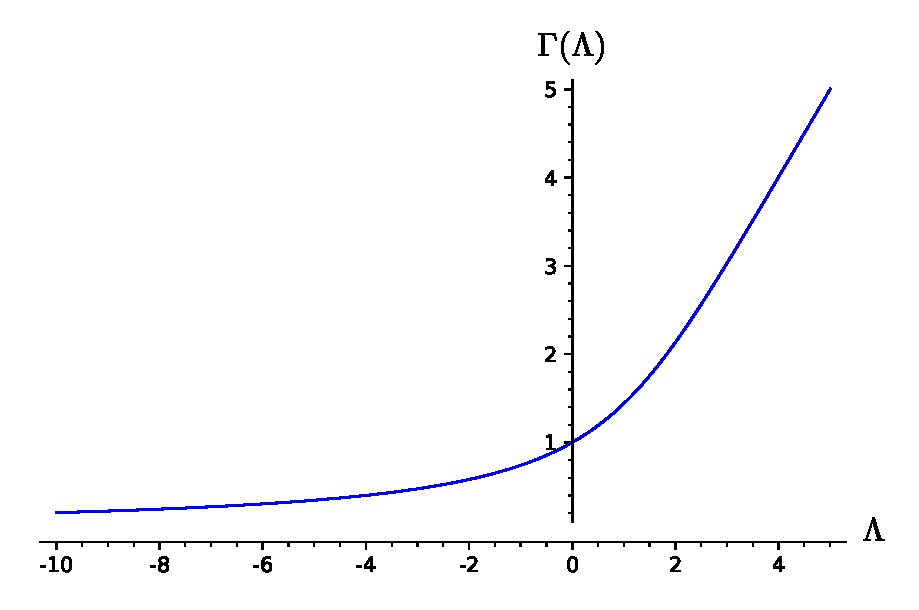
\includegraphics[width=0.5\textwidth]{gamma.eps}
\caption{Rescaled sticking term $\Gamma = (4L/l) \, \gamma$ as a function of rescaled biasing parameter $\Lambda = s L v_0/2$.}
\label{Gamma}
\end{figure}

At the lowest order in $L^{-1}$ we have from Eqs. (\ref{epsilon}, \ref{theta}, \ref{beta})
\begin{equation}
\varepsilon(r) = \theta(r) = \beta(r) = \frac{1}{2} A_+ (e^{-kr} + e^{-k(L-r)})
\end{equation}
and from Eqs. (\ref{SC1}, \ref{SC2}, \ref{SCgamma})
\begin{equation}
A_+ = \frac{2\gamma}{l} \frac{1}{1 + e^{-kL}} = \frac{k}{4(1 - e^{-kL})}
\end{equation}
so we can write with Eqs. (\ref{SCkl}, \ref{Lambda}, \ref{Phi}, \ref{eqGamma})
\begin{equation}
L \varepsilon(r) = \frac{1}{4} \Gamma \begin{cases} \frac{\cosh\left(\sqrt{\Psi}(1 - 2r/L)\right)}{\cosh\left(\sqrt{\Psi}\right)} &\text{ if } s > 0, \\ 1 &\text{ if } s = 0, \\ \frac{\cos\left(\sqrt{|\Psi|}(1 - 2r/L)\right)}{\cos\left(\sqrt{|\Psi|}\right)} &\text{ if } s < 0, \end{cases}
\end{equation}
which we plot in Fig. \ref{fig:epsilon}.

\begin{figure}[H]
\centering
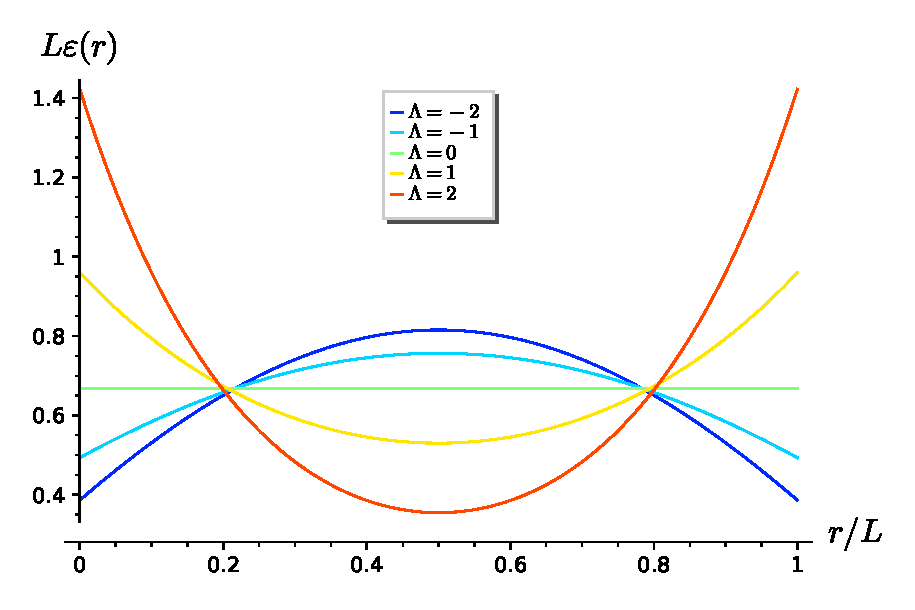
\includegraphics[width=0.5\textwidth]{epsilon.eps}
\caption{Rescaled regular part $L \varepsilon(r)$ as a function of rescaled distance $r/L$ for different values of the rescaled biasing parameter $\Lambda = s L v_0/2$.}
\label{fig:epsilon}
\end{figure}

\section{Solution to the adjoint eigenproblem}

\subsection{General solution}

We have computed the left eigenvectors $P_{\alpha_1\alpha_2}$ of Eq.~\ref{eigenproblem} corresponding to the SCGF $\psi(\lambda)$ in Sec.~\ref{sec:biased-distribution}, and will now compute the right eigenvectors $Q_{\alpha_1\alpha_2}$.
We introduce $Y_{\alpha_1\alpha_2}(r) = P_{\alpha_1\alpha_2}(r) Q_{\alpha_1\alpha_2}(r)$ which has the same symmetries as $P_{\alpha_1\alpha_2}(r)$, so that $Q_{\alpha_1\alpha_2}(r)$ also has these properties.\\

We assume that the normalisation condition
\begin{equation}
\int_0^L \sum_{\alpha_1, \alpha_2 = \pm 1} Y_{\alpha_1\alpha_2}(r) \, \mathrm{d}r = 1
\label{normalisation_pave}
\end{equation}
as well as the general form
\begin{eqnarray}
Y_{\alpha\alpha}(r) = \hat{\varepsilon}_{\alpha\alpha}(r) + \hat{\gamma}_{\alpha\alpha} \delta (r) +  \hat{\gamma}_{\alpha\alpha} \delta (L - r)\\
Y_{+-}(r) = \hat{\varepsilon}_{+-}(r) + \hat{\gamma}_{\alpha\overline{\alpha}} \delta (r)\\
Y_{-+}(r) = \hat{\varepsilon}_{-+}(r) + \hat{\gamma}_{\alpha\overline{\alpha}} \delta (L - r)
\end{eqnarray}
also hold for $Y_{\alpha_1\alpha_2}$.\\

We write the hermitian adjoints of Eqs.~\ref{FP1}, \ref{FP2}, \ref{FP3} for the right eigenvectors
\begin{eqnarray}
\label{FPr1}
\psi Q_{\alpha\alpha}(r) = -2 \partial_r V(r) \partial_r Q_{\alpha\alpha}(r) + \tau^{-1} (Q_{\alpha\overline{\alpha}}(r) + Q_{\overline{\alpha}\alpha}(r) - 2 Q_{\alpha\alpha}(r))\\
\label{FPr2}
\psi Q_{\alpha\overline{\alpha}}(r) = - \alpha 2 v_0 \partial_r Q_{\alpha\overline{\alpha}}(r) - 2 \partial_r V(r) \partial_r Q_{\alpha\overline{\alpha}}(r) + \tau^{-1} (2 Q_{\alpha\alpha}(r) - 2 Q_{\alpha\overline{\alpha}}(r)) - \alpha 2 s v_0 \partial_r V(r) Q_{\alpha\overline{\alpha}}(r)
\end{eqnarray}
following the symmetries we have introduced.\\

We notice that the bulk equations for Eqs.~\ref{FPr1}, \ref{FPr2} are the bulk equations \eqref{bulk:biased1}, \eqref{bulk:biased2}, \eqref{bulk:biased3} under the transformation $\alpha \to \overline{\alpha}$ so we get on $]0;L[$
\begin{eqnarray}
\label{qaa}
Q_{\alpha\alpha}(r) = A^{\prime} (\tau \psi + 2)^{-1} (e^{-k r} + e^{-k (L - r)})\\
\label{qaoa}
2 Q_{\alpha\overline{\alpha}}(r) = \left(1 + \frac{\alpha 2 k l}{\tau \psi + 2}\right) A^{\prime} e^{- k r} + \left(1 - \frac{\alpha 2 k l}{\tau \psi + 2}\right) A^{\prime} e^{- k (L - r)}
\end{eqnarray}
where $k$ is defined by Eq.~\ref{kPsi} and $A^{\prime}$ is a new constant.\\

We write for $Y_{\alpha_1\alpha_2}$ the equations
\begin{eqnarray}
\label{FPrY1}
\begin{aligned}
\psi Y_{\alpha\overline{\alpha}}(r) \frac{P_{\alpha\alpha}(r)}{P_{\alpha\overline{\alpha}}(r)} = &\left[- \alpha 2 v_0 \partial_r Q_{\alpha\overline{\alpha}}(r) - 2 \partial_r V(r) \partial_r Q_{\alpha\overline{\alpha}}(r)\right] P_{\alpha\alpha}(r)\\
&+ \tau^{-1} \left(2 Y_{\alpha\alpha}(r) - 2 Y_{\alpha\overline{\alpha}}(r) \frac{P_{\alpha\alpha}(r)}{P_{\alpha\overline{\alpha}}(r)}\right) - \alpha 2 s v_0 \partial_r V(r) Y_{\alpha\overline{\alpha}}(r) \frac{P_{\alpha\alpha}(r)}{P_{\alpha\overline{\alpha}}(r)}
\end{aligned}\\
% \label{FPrY1}
% \psi Y_{\alpha\alpha}(r) = - 2 \partial_r V(r) P_{\alpha\alpha}(r) \partial_r Q_{\alpha\alpha}(r) + \tau^{-1} \left(Y_{\alpha\overline{\alpha}}(r) \frac{P_{\alpha\alpha(r)}}{P_{\alpha\overline{\alpha}}(r)} + Y_{\overline{\alpha}\alpha}(r) \frac{P_{\alpha\alpha(r)}}{P_{\overline{\alpha}\alpha}(r)} - 2 Y_{\alpha\alpha}(r)\right)\\
% \label{FPrY2}
% \psi Y_{\alpha\alpha}(r) = 2 Q_{\alpha\alpha}(r) \partial_r (P_{\alpha\alpha}(r) \partial_r V(r)) + \tau^{-1} \left(Y_{\alpha\alpha}(r) \frac{P_{\alpha\overline{\alpha}}(r)}{P_{\alpha\alpha}(r)} + Y_{\alpha\alpha}(r) \frac{P_{\overline{\alpha}\alpha}(r)}{P_{\alpha\alpha}(r)} - 2 Y_{\alpha\alpha}(r)\right)\\
\label{FPrY3}
\begin{aligned}
\psi Y_{\alpha\overline{\alpha}}(r) = &- \alpha 2 v_0 P_{\alpha\overline{\alpha}}(r) \partial_r Q_{\alpha\overline{\alpha}}(r) - 2 \partial_r V(r) P_{\alpha\overline{\alpha}}(r) \partial_r Q_{\alpha\overline{\alpha}}(r) + \tau^{-1} \left(2 Y_{\alpha\alpha}(r) \frac{P_{\alpha\overline{\alpha}}(r)}{P_{\alpha\alpha}(r)} - 2 Y_{\alpha\overline{\alpha}}(r)\right)\\
&- \alpha 2 s v_0 \partial_r V(r) Y_{\alpha\overline{\alpha}}(r)
\end{aligned}\\
\label{FPrY4}
\begin{aligned}
\psi Y_{\alpha\overline{\alpha}}(r) = &\alpha 2 v_0 Q_{\alpha\overline{\alpha}}(r) \partial_r P_{\alpha\overline{\alpha}}(r) + 2 Q_{\alpha\overline{\alpha}}(r) \partial_r (Q_{\alpha\overline{\alpha}}(r) \partial_r V(r)) + \tau^{-1} \left(2 Y_{\alpha\overline{\alpha}}(r) \frac{P_{\alpha\alpha}(r)}{P_{\alpha\overline{\alpha}}(r)} - 2 Y_{\alpha\overline{\alpha}}(r)\right)\\
&- \alpha 2 s v_0 \partial_r V(r) Y_{\alpha\overline{\alpha}}(r)
\end{aligned}
\end{eqnarray}
where \eqref{FPrY1} is derived from the multiplication of \eqref{FPr2} by $P_{\alpha\alpha}(r)$,
% where \eqref{FPrY1} is derived from the multiplication of \eqref{FPr1} by $P_{\alpha\alpha}(r)$, \eqref{FPrY2} is derived from the multiplication of \eqref{FP1} by $Q_{\alpha\alpha}(r)$,
\eqref{FPrY3} is derived from the multiplication of \eqref{FPr2} by $P_{\alpha\overline{\alpha}}(r)$, \eqref{FPrY4} is derived from the multiplication of (\ref{FP2}, \ref{FP3}) by $Q_{\alpha\overline{\alpha}}(r)$
, and finally substract
%
% We substract Eqs.~\ref{FPrY1},~\ref{FPrY2}
% \begin{equation}
% 0 = - 2 \partial_r (\partial_r V(r) Y_{\alpha\alpha}(r)) + \tau^{-1} \left(Y_{\alpha\overline{\alpha}}(r) \frac{P_{\alpha\alpha(r)}}{P_{\alpha\overline{\alpha}}(r)} + Y_{\overline{\alpha}\alpha}(r) \frac{P_{\alpha\alpha(r)}}{P_{\overline{\alpha}\alpha}(r)} - Y_{\alpha\alpha}(r) \frac{P_{\alpha\overline{\alpha}}(r)}{P_{\alpha\alpha}(r)} - Y_{\alpha\alpha}(r) \frac{P_{\overline{\alpha}\alpha}(r)}{P_{\alpha\alpha}(r)}\right)
% \end{equation}
% and also
Eqs.~\ref{FPrY3},~\ref{FPrY4}
\begin{equation}
0 = - \alpha 2 v_0 \partial_r Y_{\alpha\overline{\alpha}}(r) - 2 \partial_r (Y_{\alpha\overline{\alpha}}(r) \partial_r V(r)) + \tau^{-1} \left(2 Y_{\alpha\alpha}(r) \frac{P_{\alpha\overline{\alpha}}(r)}{P_{\alpha\alpha}(r)} - 2 Y_{\alpha\overline{\alpha}}(r) \frac{P_{\alpha\alpha}(r)}{P_{\alpha\overline{\alpha}}(r)}\right)
\end{equation}
to get equations where derivatives should have nice integrals.\\

We integrate Eqs.~\ref{FPrY1},~\ref{FPrY4} between $0^-$ and $0^+$
\begin{eqnarray}
\label{BCr1}
\psi \hat{\gamma}_{\alpha\overline{\alpha}} \frac{\gamma_{\alpha\alpha}}{\gamma_{\alpha\overline{\alpha}}} = \tau^{-1} \left(2 \hat{\gamma}_{\alpha\alpha} - 2 \hat{\gamma}_{\alpha\overline{\alpha}} \frac{\gamma_{\alpha\alpha}}{\gamma_{\alpha\overline{\alpha}}}\right) + 2 s v_0^2 \hat{\gamma}_{\alpha\overline{\alpha}} \frac{\gamma_{\alpha\alpha}}{\gamma_{\alpha\overline{\alpha}}}\\
\label{BCr2}
0 = - v_0 \hat{\varepsilon}_{+-}(0^+) + \tau^{-1} \left(\hat{\gamma}_{\alpha\alpha} \frac{\gamma_{\alpha\overline{\alpha}}}{\gamma_{\alpha\alpha}} - \hat{\gamma}_{\alpha\overline{\alpha}} \frac{\gamma_{\alpha\alpha}}{\gamma_{\alpha\overline{\alpha}}}\right)
\end{eqnarray}
where we have discarded in \eqref{BCr1} the integral of the first term of the right hand side of \eqref{FPrY1} since $\partial_r V(0) = -v_0$, and where
\begin{eqnarray}
\label{he+-}
\begin{aligned}
\hat{\varepsilon}_{+-}(r) &= Q_{+-}(r) P_{+-}(r) \qquad (r \in ]0; L[)\\
&= \frac{A A^{\prime}}{4} \left[1 - \left(\frac{2 k l}{\tau \psi + 2}\right)^2\right](e^{-2 k r} + e^{-2 k (L - r)}) + \frac{A A^{\prime}}{4} \left[\left(1 + \frac{2 k l}{\tau \psi + 2}\right)^2 + \left(1 - \frac{2 k l}{\tau \psi + 2}\right)^2\right] e^{-k L}
\end{aligned}\\
\label{he+-lim}
\begin{aligned}
\hat{\varepsilon}_{+-}(0^+) = \lim_{r \to 0^+} \hat{\varepsilon}_{+-}(r) = \frac{A A^{\prime}}{4} \left[1 - \left(\frac{2 k l}{\tau \psi + 2}\right)^2\right](1 + e^{-2 k L}) + \frac{A A^{\prime}}{4} \left[\left(1 + \frac{2 k l}{\tau \psi + 2}\right)^2 + \left(1 - \frac{2 k l}{\tau \psi + 2}\right)^2\right] e^{-k L}
\end{aligned}
\end{eqnarray}
from Eqs.~\ref{epsilon},~\ref{qaoa}, with $A = A_{\pm}$ which appear in Eqs.~\ref{epsilon}, \ref{theta}, \ref{beta}. We solve Eqs.~\ref{BCr1},~\ref{BCr2} for $\hat{\gamma}_{\alpha\alpha}$ and $\hat{\gamma}_{\alpha\overline{\alpha}}$
\begin{eqnarray}
\label{hgaa}
\hat{\gamma}_{\alpha\alpha} = \frac{\left[\frac{1}{2} (\tau \psi + 2) - s l v_0\right] \frac{\gamma_{\alpha\alpha}}{\gamma_{\alpha\overline{\alpha}}} l \hat{\varepsilon}_{+-}(0^+)}{\frac{1}{2}(\tau\psi + 2) - s l v_0 - \frac{\gamma_{\alpha\alpha}}{\gamma_{\alpha\overline{\alpha}}}}\\
\label{hgaoa}
\hat{\gamma}_{\alpha\overline{\alpha}} = \frac{l \hat{\varepsilon}_{+-}(0^+)}{\frac{1}{2}(\tau\psi + 2) - s l v_0 - \frac{\gamma_{\alpha\alpha}}{\gamma_{\alpha\overline{\alpha}}}}
\end{eqnarray}
as a function of $\hat{\varepsilon}_{+-}(0^+)$.\\

We can finally write the normalisation condition \eqref{normalisation_pave}
\begin{equation}
1 = 4 \hat{\gamma}_{\alpha\alpha} + 2 \hat{\gamma}_{\alpha\overline{\alpha}} + 2 \int_0^L \hat{\varepsilon}_{\alpha\alpha}(r) \, \mathrm{d}r + 2 \int_0^L \hat{\varepsilon}_{\alpha\overline{\alpha}}(r) \, \mathrm{d}r
\label{normalisation_pave_full}
\end{equation}
where we have
\begin{equation}
\hat{\varepsilon}_{\alpha\alpha}(r) = P_{\alpha\alpha}(r \in ]0; L[) Q_{\alpha\alpha}(r \in ]0; L[) = \frac{A A^{\prime}}{(\tau \psi + 2)^2} \left(e^{-2 k r} + e^{-2 k (L - r)} + 2 e^{-k L}\right)
\label{heaa}
\end{equation}
according to Eqs.~\ref{beta},~\ref{qaa}. We can then finally determine $A^{\prime}$ from (\ref{he+-}, \ref{he+-lim}, \ref{hgaa}, \ref{hgaoa}, \ref{normalisation_pave_full}, \ref{heaa}) and thus know $Y_{\alpha_1\alpha_2}$ completely.

\subsection{Unbiased ensemble check}

We have in the unbiased ensemble $\psi(s = 0) = 0$, therefore $k = 0$ according to \eqref{kPsi}. It follows that
\begin{equation}
\hat{\varepsilon}_{\alpha\alpha}(r, s=0) = \hat{\varepsilon}_{\alpha\overline{\alpha}}(r, s=0) = A A^{\prime}
\end{equation}
from Eqs.~\ref{he+-},~\ref{heaa}. We know from Eqs.~\ref{s0++}, \ref{s0--}, \ref{s0+-}, \ref{s0-+} that
\begin{equation}
\left. \frac{\gamma_{\alpha\alpha}}{\gamma_{\alpha\overline{\alpha}}} \right|_{s=0} = \frac{1}{2}
\end{equation}
therefore we get
\begin{eqnarray}
\hat{\gamma}_{\alpha\alpha}(s=0) = l A A^{\prime}\\
\hat{\gamma}_{\alpha\overline{\alpha}}(s=0) = 2 l A A^{\prime}
\end{eqnarray}
from Eqs.~\ref{hgaa},~\ref{hgaoa}. We can then write the normalisation condition \eqref{normalisation_pave_full}
\begin{equation}
1 = 4 l A A^{\prime} + 4 l A A^{\prime} + 2 A A^{\prime} L + 2 A A^{\prime} L
\end{equation}
such that
\begin{equation}
A^{\prime} = \frac{1}{A( 8 l + 4 L)} = 1
\end{equation}
where the second equality derives from Eq.~\ref{smooth_unbiased}, and which consequence is that
\begin{equation}
Q_{\alpha\alpha}(r, s=0) = Q_{\alpha\overline{\alpha}}(r, s=0) = 1
\end{equation}
according to Eqs.~\ref{qaa},~\ref{qaoa}.

%%%%%%%%%%%%%%
% REFERENCES %
%%%%%%%%%%%%%%

\bibliographystyle{alpha}
{\renewcommand{\bibname}{References}\bibliography{references}}

\end{document}
